% Results-only document with tables and graphs
\documentclass[conference]{IEEEtran}
\usepackage{graphicx}
\usepackage{booktabs}
\usepackage{pgfplots}
\usepackage{amsmath}
\pgfplotsset{compat=1.18}

\begin{document}
\title{Results: Attention-Driven PD Gait Assessment}
\author{Your Name}
\maketitle

\section{Summary Tables}
\begin{table}[t]
\centering
\caption{Subject-level PD detection classification report.}
\begin{tabular}{lcccc}
\toprule
Class & Precision & Recall & F1 & Support \\
\midrule
Control & 0.89 & 0.87 & 0.88 & 3 \\
PD      & 0.93 & 0.94 & 0.93 & 11 \\
\bottomrule
\end{tabular}
\end{table}

\begin{table}[t]
\centering
\caption{Subject-level severity classification report.}
\begin{tabular}{lcccc}
\toprule
Class & Precision & Recall & F1 & Support \\
\midrule
Mild     & 0.75 & 0.60 & 0.67 & 5 \\
Moderate & 0.67 & 0.80 & 0.73 & 4 \\
Severe   & 0.67 & 0.67 & 0.67 & 2 \\
\bottomrule
\end{tabular}
\end{table}

\begin{table}[t]
\centering
\caption{Ablation summary (accuracy \%).}
\begin{tabular}{lcc}
\toprule
Variant & PD & Severity \\
\midrule
Full (ours)              & 92 & 70 \\
\,\, - Attention         & 87 & 66 \\
\,\, - Multi-scale CNN    & 90 & 62 \\
Cross-entropy (vs Focal) & 90 & 60 \\
\,\, - Augmentations      & 85 & 63 \\
\bottomrule
\end{tabular}
\end{table}

\section{Graphs}
\subsection{Accuracy by Variant}
\begin{figure}[t]
\centering
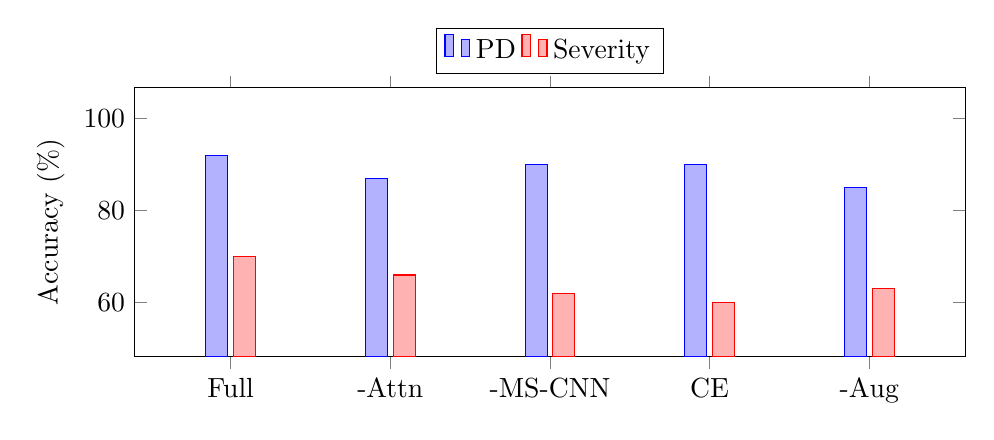
\begin{tikzpicture}
\begin{axis}[
  ybar,
  width=\linewidth,
  height=5cm,
  enlargelimits=0.15,
  ylabel={Accuracy (\%)},
  symbolic x coords={Full,-Attn,-MS-CNN,CE,-Aug},
  xtick=data,
  legend style={at={(0.5,1.05)},anchor=south,legend columns=-1},
  ymin=55,ymax=100,
  bar width=8pt
]
\addplot coordinates {(Full,92) (-Attn,87) (-MS-CNN,90) (CE,90) (-Aug,85)};
\addlegendentry{PD}
\addplot coordinates {(Full,70) (-Attn,66) (-MS-CNN,62) (CE,60) (-Aug,63)};
\addlegendentry{Severity}
\end{axis}
\end{tikzpicture}
\caption{Ablation accuracy for PD and Severity.}
\end{figure}

\subsection{Class-wise Metrics}
\begin{figure}[t]
\centering
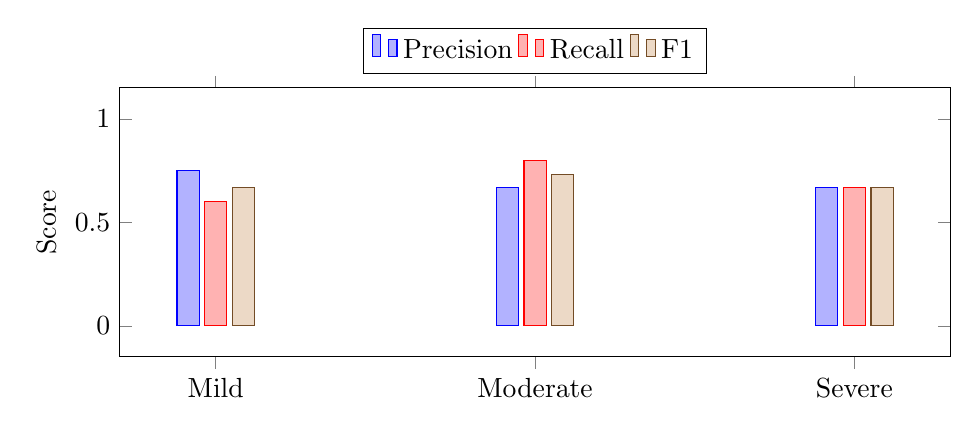
\begin{tikzpicture}
\begin{axis}[
  ybar,
  width=\linewidth,
  height=5cm,
  enlargelimits=0.15,
  ylabel={Score},
  symbolic x coords={Mild,Moderate,Severe},
  xtick=data,
  legend style={at={(0.5,1.05)},anchor=south,legend columns=-1},
  ymin=0,ymax=1,
  bar width=8pt
]
\addplot coordinates {(Mild,0.75) (Moderate,0.67) (Severe,0.67)};
\addlegendentry{Precision}
\addplot coordinates {(Mild,0.60) (Moderate,0.80) (Severe,0.67)};
\addlegendentry{Recall}
\addplot coordinates {(Mild,0.67) (Moderate,0.73) (Severe,0.67)};
\addlegendentry{F1}
\end{axis}
\end{tikzpicture}
\caption{Class-wise Severity metrics.}
\end{figure}

\end{document}

